Time series are generated and stored at a vastly increasing rate in many industrial and research applications, including the Web and the Internet of Things, public utilities, finance, astronomy, biology, and many more. A significant portion concerns \emph{geolocated} time series, i.e., those generated at, or otherwise associated with, specific locations. While indexing, mining and exploring time series data has attracted a lot of interest from the database and data mining communities \cite{camerra2014kais,ding2008pvldb,shieh2008kdd}, studying of geolocated time series is still largely overlooked.

Geolocated time series can be found in various domains and applications. For instance, time series can be used to represent, analyze and forecast water consumption measured by smart meters installed in urban households \cite{DBLP:conf/edbt/ChronisGA16}. Analyzing such time series can provide valuable insights regarding trends and patterns of consumer behavior in daily life. These results can then be used to forecast and balance water demand, as well as to plan and prioritize interventions that can guide consumers towards more sensible water use. Similar use cases can be found in other domains, such as in geomarketing or mobile advertisement, where geolocated time series may represent the number of visitors or the revenue generated at a certain location across time. Extracting insights, trends and patterns can be significantly facilitated by {\em map-based visualizations} of {\em summarized} time series data. Such visualizations can reveal, for instance, which type of consumption patterns are most frequently observed among consumers in a certain area or what the spatial distribution of sales for a certain product looks like. 

However, time series is an inherently complex data type, and such datasets can reach extremely large volumes, both {\em horizontally} (i.e., very long series of values across time) and {\em vertically} (i.e., time series generated by countless sources). Consequently, management, analysis and exploration of big time series data is a task requiring efficient and scalable algorithms. In particular, visual exploration of geolocated time series needs to process the required information efficiently, while the user interacts with the application. For example, whenever the user zooms in or scrolls the map, visual analytics and aggregates should be computed on-the-fly, e.g., identifying the predominant patterns in the time series and their spatial distribution within the actual map area.

Consider the example illustrated in Figure~\ref{subfig:map}. When the user zooms the map into the red rectangle, the visualization application should identify, summarize and present the two patterns (shown in blue and green color) appearing therein. For such requests that inherently combine spatial filters with time series analysis, it is inefficient to evaluate each predicate separately, e.g., apply a spatial filter on the time series of a large dataset and then calculate summaries of the candidates, or vice versa. The same stands for the case of exploration on the time series domain, as depicted in Figure~\ref{subfig:timebox}. Consider a user drawing a {\em timebox} (i.e., a rectangle in the time series domain) or zooming in the yellow part. The application should identify the time series that are fully contained within that filter area, i.e., their values along the specified time range fall within the value range (both ranges shown in orange in Figure~\ref{subfig:timebox}), and then provide an informative summary comprising aggregate spatial information to avoid cluttering the map.

\begin{figure}[!t]
 \centering
 \subfloat[Exploring time series patterns in a {\em spatial region}.] {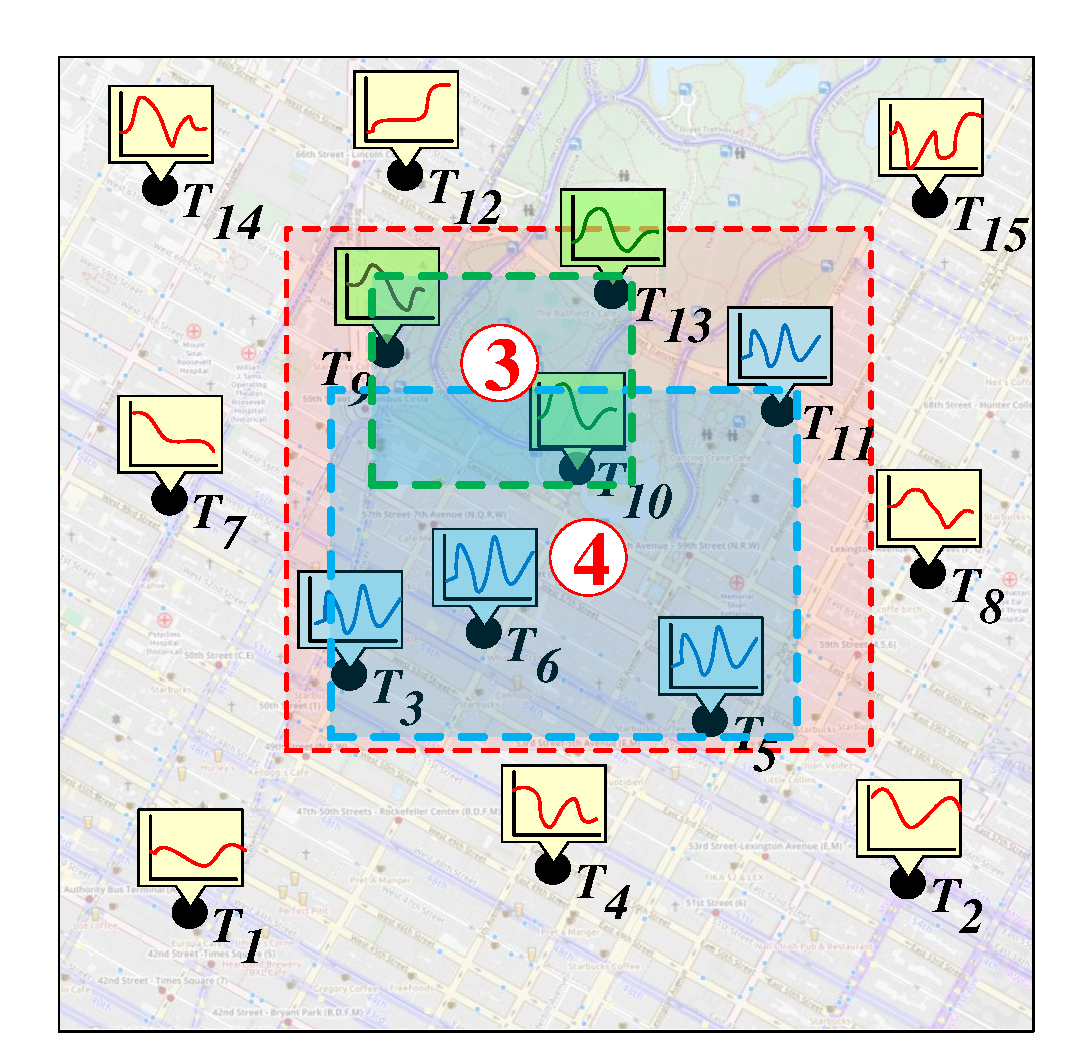
\includegraphics[width=0.375\textwidth]{figures/map2.pdf}\label{subfig:map}}
 \subfloat[Exploring time series in a {\em timebox} of interest.]{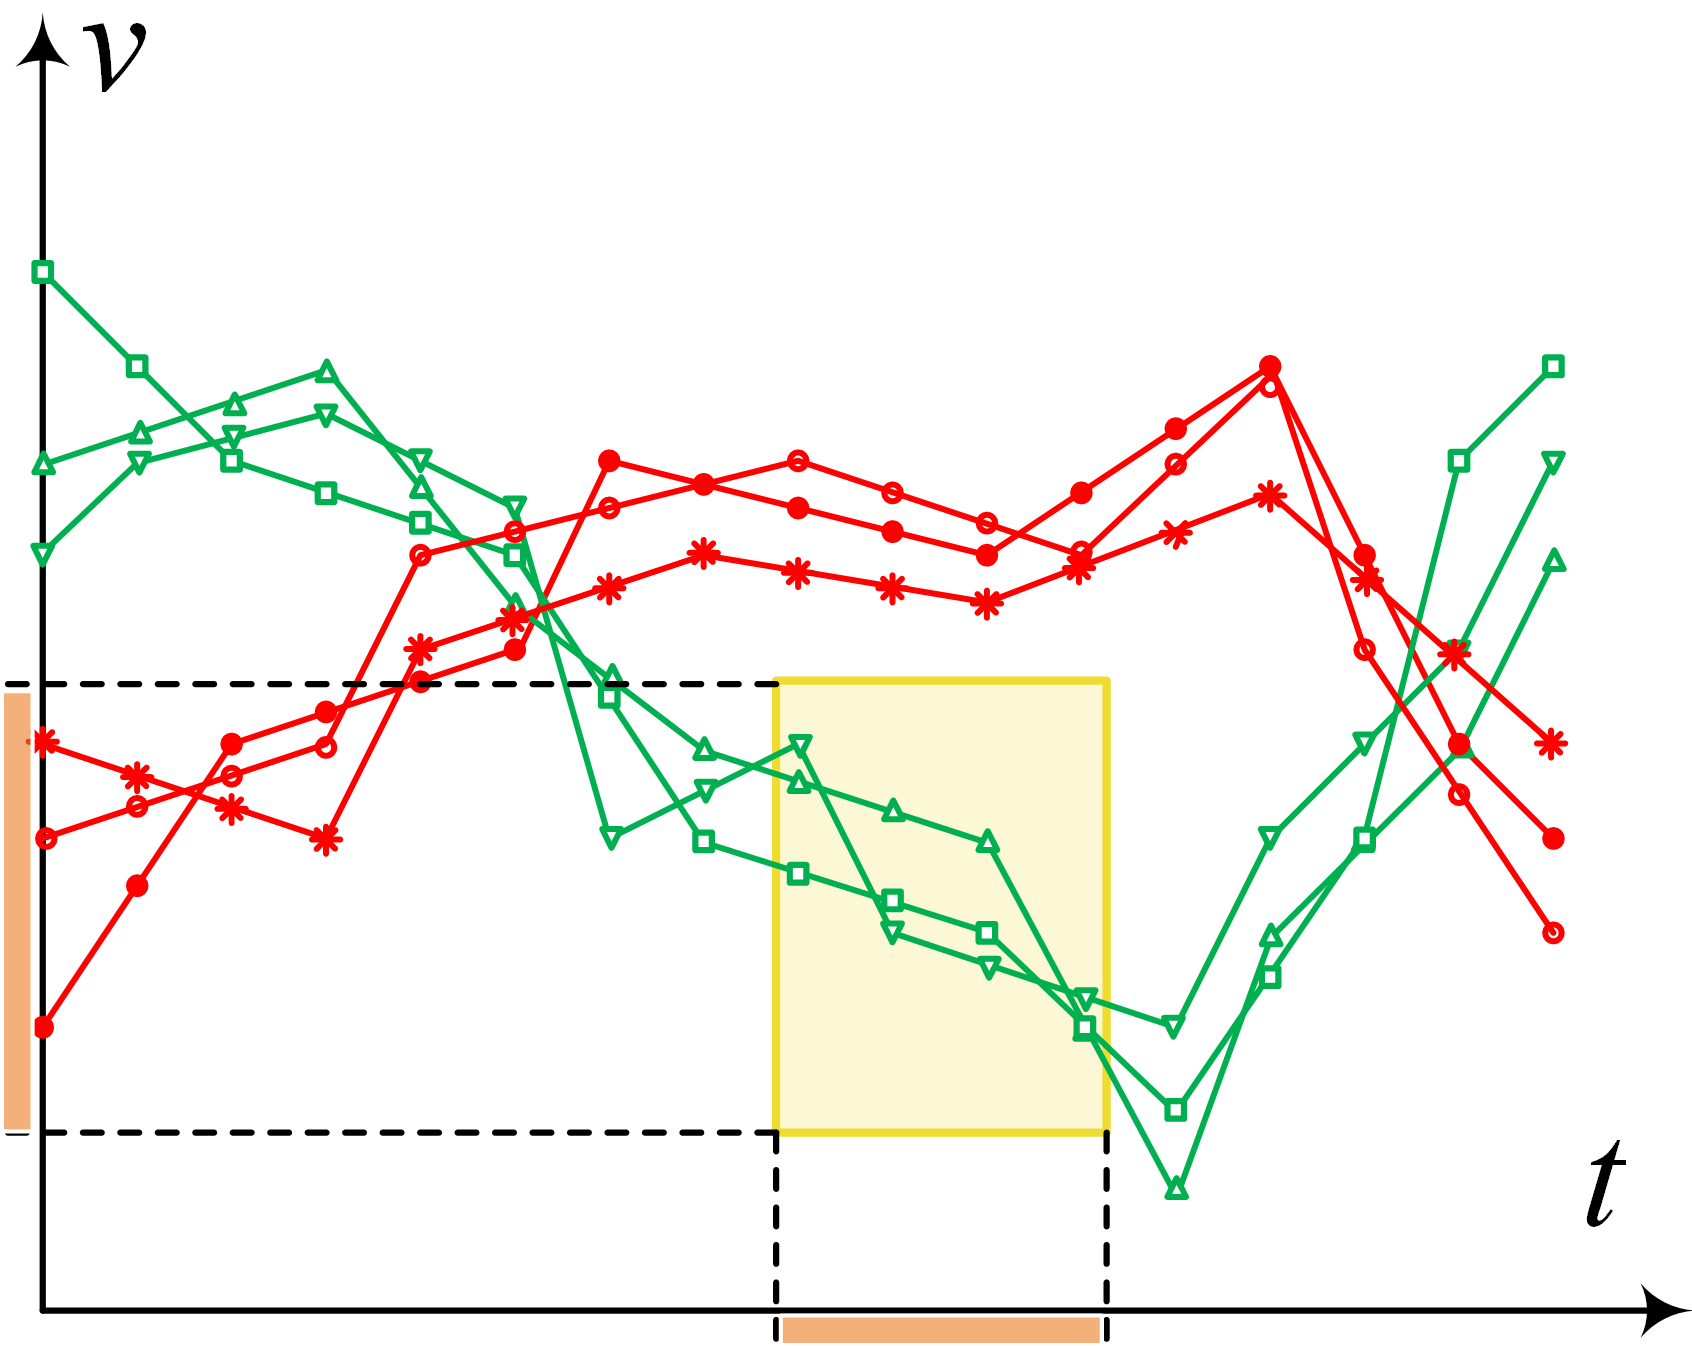
\includegraphics[width=0.45\textwidth]{figures/timebox.png}\label{subfig:timebox}}\
\caption{Visual exploration examples over geolocated time series.}
\label{fig:examples}
\end{figure}

Efficient filtering and retrieval over large datasets of geolocated time series can be enabled by {\em indexing}. Several approaches have been proposed that efficiently index large amounts of plain time series data. They either rely on \emph{Discrete Wavelet Transform} to reduce the dimensionality of time series \cite{chan1999icde}, or make use of a family of indices based on \emph{Symbolic Aggregate Approximation} (SAX) \cite{shieh2008kdd,camerra2010icdm,camerra2014kais,zoumpatianos2014sigmod}. However, all aforementioned techniques index the data solely on the time series domain, not taking the spatial dimension into account. If each analyzed time series is inherently associated with a spatial attribute (e.g., locations of smart meters), such indexing is not sufficient for queries and visualizations that additionally involve spatial filters.

In this paper, we propose two geolocated time series summarization approaches for visual exploration, named {\em bundle} and {\em tile map summary}. These are supported and driven by two appropriate {\em hybrid} indices that speed up the result computation, providing efficient exploration of geolocated time series data. They consist of a spatial and a time series summary that jointly facilitate knowledge extraction and insight gaining. The spatial summary is similar for both and consists of {\em Minimum Bounding Rectangles} (MBRs) of geolocated time series, according to a specific predicate (i.e., spatial proximity, or time series similarity). Each MBR is associated with a counter denoting the number of time series it contains. A visualization example of the spatial summary is depicted in Figure~\ref{subfig:map}, where the geolocated time series are organized in two groups (i.e., green and blue colored) according to their similarity. Each group is depicted along with a number that indicates the amount of time series that it contains (i.e., three geolocated time series for the first group and four for the second).

The main difference among the two methods lies in the time series part of the summary. The bundle summary consists of sets of {\em Minimum Bounding Time Series} (MBTS)~\cite{chatzig17btsr}, an example of which is depicted in Figure~\ref{subfig:bundle}. An MBTS is a band with upper and lower bounds that encloses all time series of a set, providing with a notion of a range of the time series values throughout the time axis. On the other hand, the tile map summary (Figure~\ref{subfig:tile_map}) of a set of time series indicates (using a corresponding shading), the density of the time series points at each tile of a partitioning of the domain, obtained by discretizing the time and value axes. This way, it avoids overplotting that would be caused by outputting a large number of resulting time series and provides a notion of how the values of the time series are distributed across time.

\begin{figure}[!t]
 \centering
 \subfloat[Bundle summary.]{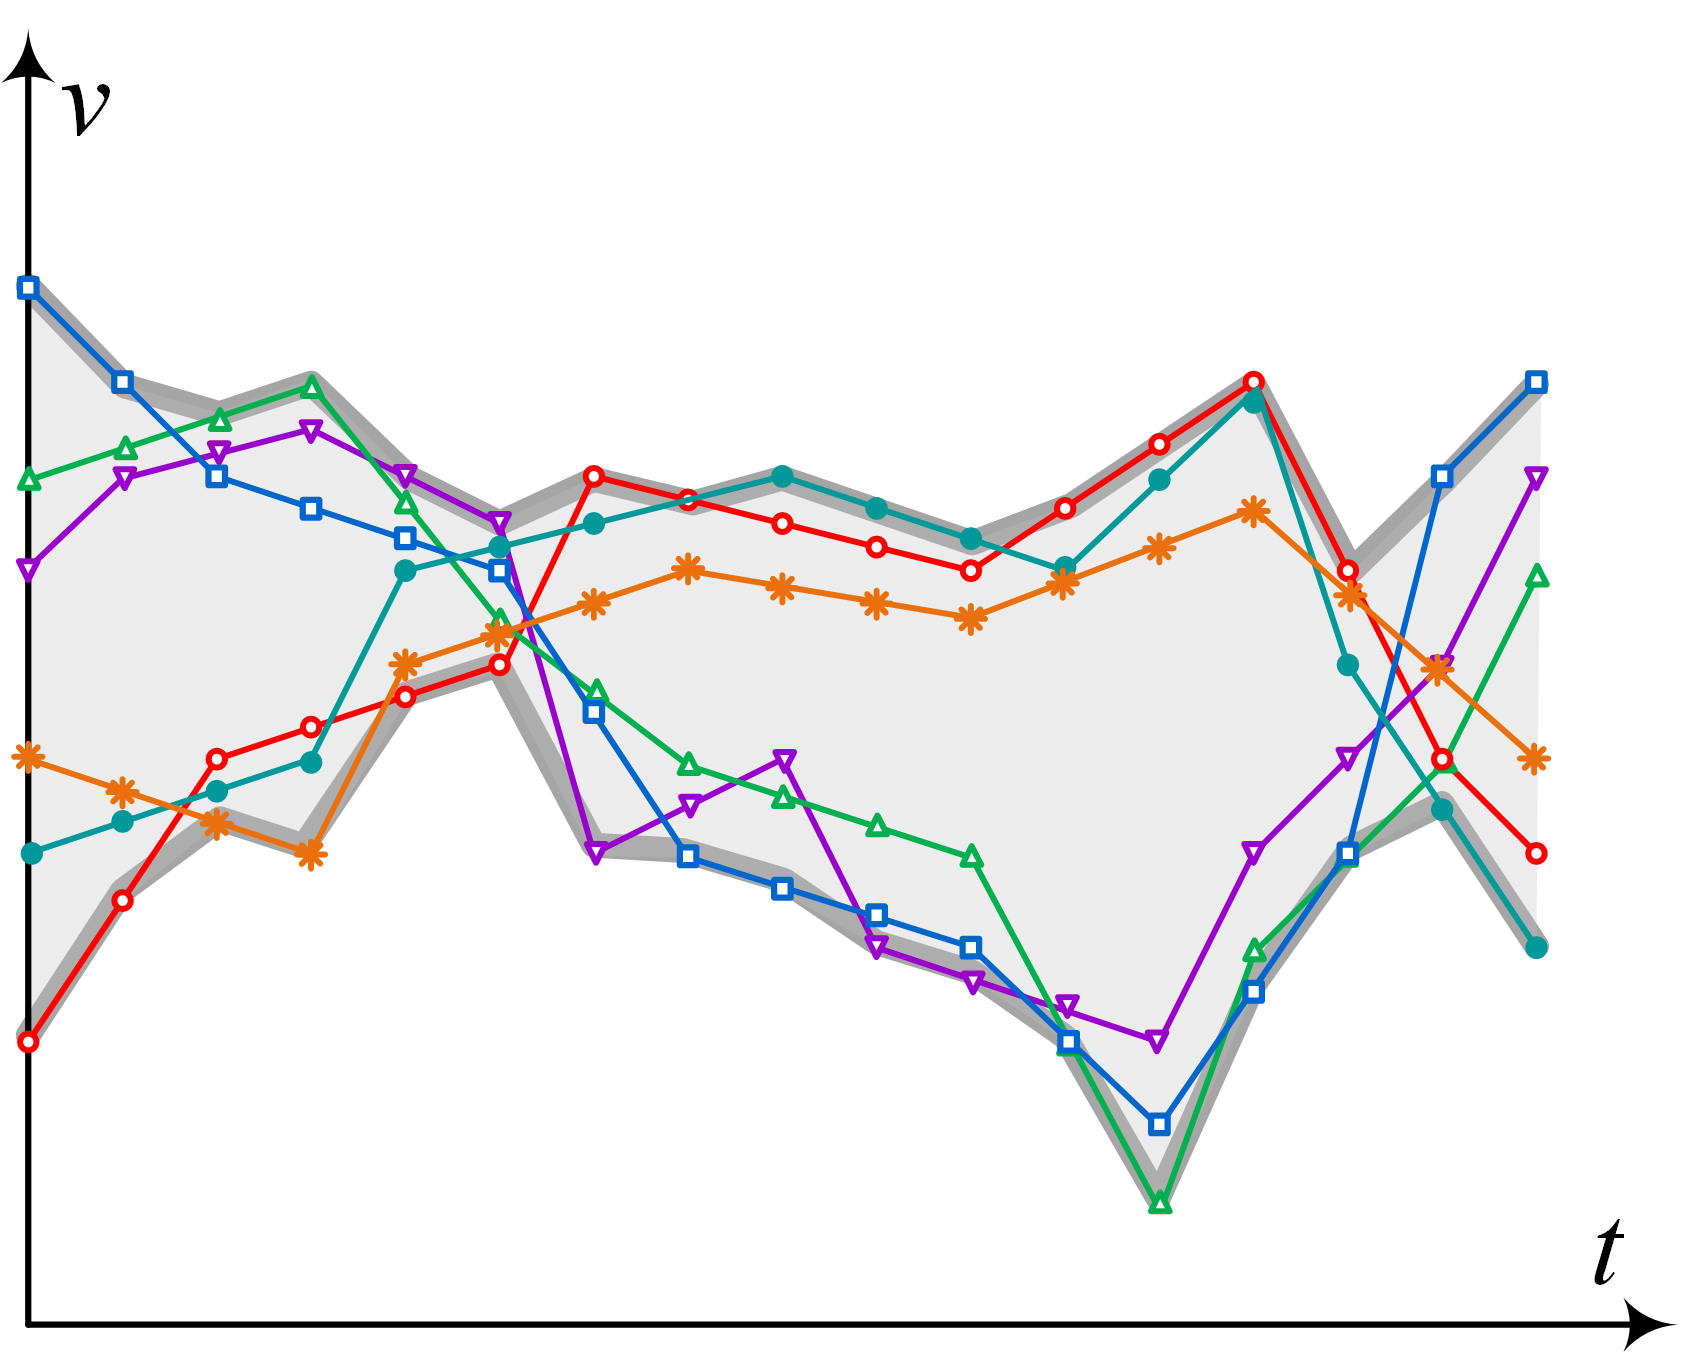
\includegraphics[width=0.45\textwidth]{figures/bounds_tsr.png}\label{subfig:bundle}}
 \subfloat[Tile map summary.]{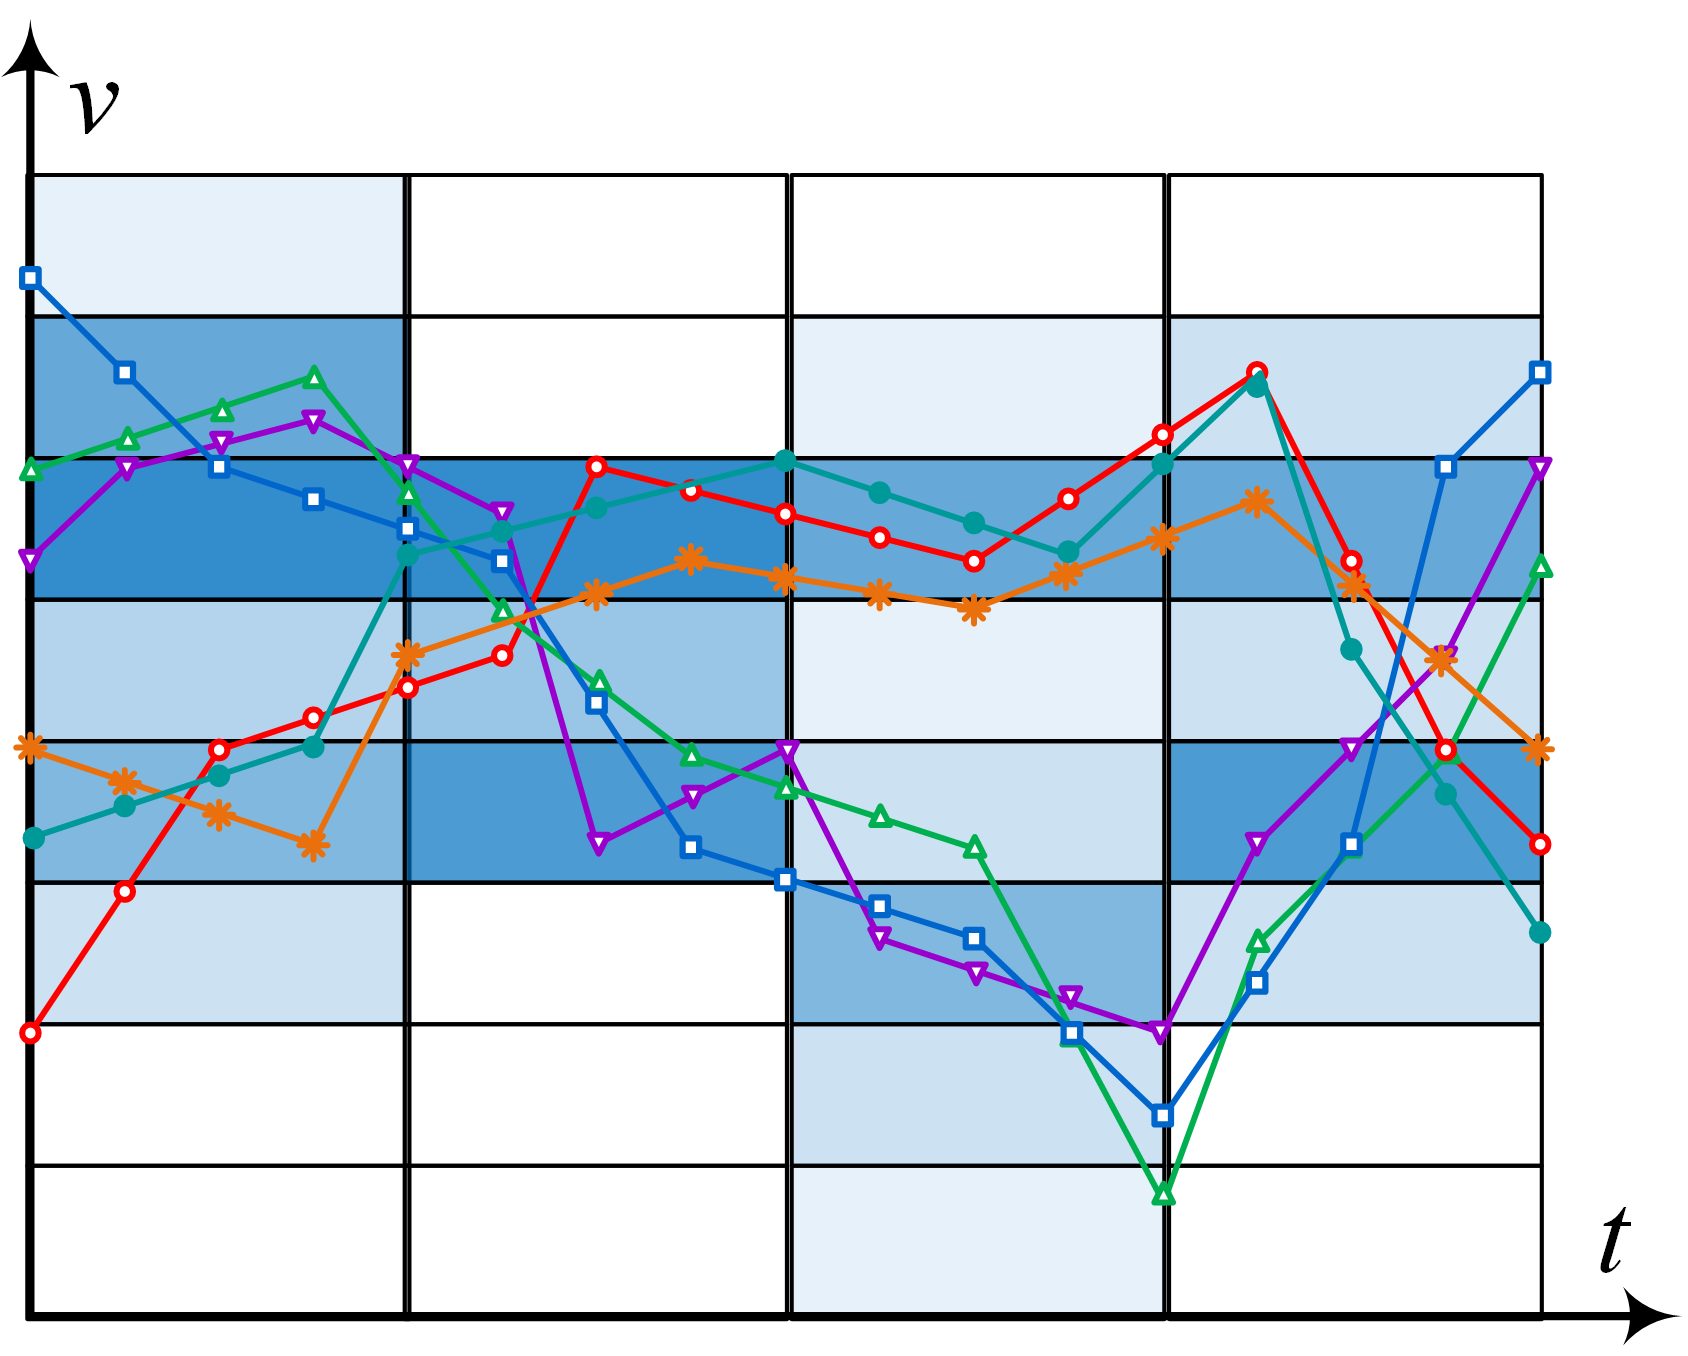
\includegraphics[width=0.45\textwidth]{figures/tile_map.png}\label{subfig:tile_map}}\
\caption{Examples of computed summaries on the time series domain.}
\label{fig:examples2}
\end{figure}

The bundle summary is driven by our recently proposed {\em \btsr} index \cite{chatzig17btsr}. This is a {\em spatial-first} hybrid index, in the sense that it is primarily built on the spatial attribute of the data. More specifically, it is an extension of the R-tree spatial index \cite{Guttman1984}, offering efficient support for similarity search over geolocated time series. The idea behind the \btsr index is to combine both spatial proximity and time series similarity. To that end, in addition to the standard MBR denoting the spatial bound of its contents, each node is augmented with an MBTS of all the time series contained in its subtree. Maintaining both kinds of bounds per node enables pruning the search space simultaneously in the spatial and the time series domains while traversing the index. To increase pruning effectiveness, the time series indexed in a given node are further distinguished into {\em bundles} on the basis of their similarity, hence achieving tighter bounds in the MBTS of these bundles. For providing prompt visualizations of summaries over geolocated time series data and minimizing latency when drawing the relevant graphic elements, we need early access to both spatial and time series information while traversing the index. For this purpose, we adapt the \btsr index so as to also include {\em aggregates} per node, i.e., the number of time series pertaining to each bundle. Subsequently, we introduce a new traversal algorithm for efficient retrieval of a given number of bundles that are the most representative in the map area. 

The tile map summary is driven by \hisax, a hybrid index we introduce in this paper. This is a {\em time series-first} index, i.e., it is primarily built in the time series domain. More specifically, it constitutes a hybrid variant of the \isax index \cite{shieh2008kdd,camerra2010icdm,camerra2014kais}, augmented with spatial attributes of its nodes' children, to combine spatial and time series information. In each node, besides the SAX word that describes all its children time series, \hisax keeps also the MBR that they form. To minimize the size and overlap of the MBRs, we propose a spatial splitting policy, that instead of choosing the splitting dimension in a round-robin fashion (as in \isax), it does so by selecting the dimension that produces the smallest overlap and overall size of the two generated MBRs. We introduce a traversal algorithm for applying timebox search on large (both vertically and horizontally) geolocated time series datasets. The traversal algorithm is applied on our \hisax index and returns a tile map-like summary of the qualifying geolocated time series, by taking advantage of the SAX representation's properties.

To the best of our knowledge, this is the first work that considers visual exploration and summarization of geolocated time series. Specifically, we propose two summarization methods enabling efficient map-based exploration driven by suitable hybrid indices. The work in this paper builds upon and extends our effort in~\cite{chatzigeorgakidis2018map}, which showed the benefits of using \btsr for visual exploration of geolocated time series. Here, we introduce another novel summarization approach that enables a different exploration method, by employing a time series-first hybrid index. In brief, our main contributions are as follows:

\begin{itemize}
 \item We suggest an adapted variant of the \btsr index, as well as a novel algorithm for its traversal in order to quickly retrieve summaries (a.k.a. bundles) of geolocated time series within a given spatial area.
 \item We propose a hybrid variant of the \isax index, called \hisax, which combines time series with spatial information within its nodes. Based on that, we describe a novel traversal algorithm for \hisax that enables fast timebox search by performing efficient pruning, while avoiding false negatives.
 \item We exemplify the proposed visualization methods with two use cases based on real-world datasets. In addition, we empirically evaluate the performance of our summarization methods, confirming their low execution time against a large synthetic dataset of geolocated time series.
\end{itemize}

The remainder of this paper is organized as follows. Section~\ref{sec:related} reviews related work. %Section~\ref{sec:preliminaries} provides background on visualization and indexing approaches that we employ. 
Section~\ref{sec:problem} outlines basic concepts and formulates the problem. Sections~\ref{sec:bundles_summary} and \ref{sec:tilemap_summary} introduce our methods for efficient visual exploration of geolocated time series by harnessing the potential of the \btsr and \hisax indices, respectively. Section~\ref{sec:evaluation} presents indicative use cases with map visualizations and also reports performance results from our empirical study. Finally, Section~\ref{sec:conclusions} concludes the paper and outlines future research directions.